\subsubsection{Runtime System for Application-Level Power Steering on Exascale Systems} 

\paragraph{Overview} 
Power remains a critical constraint for Exascale. As we design supercomputers at larger scales, power becomes an expensive and limited resource. Inefficient management of power leads to added operational costs as well as low scientific throughput. Although hardware advances will contribute a certain amount towards achieving high energy efficiency, they will not be sufficient, creating a need for a sophisticated system software approach. Significant advances in software technologies are thus required to ensure that Exascale systems achieve high performance with effective utilization of available power. Distributing available power to nodes while adhering to system, job and node constraints involves complex decision making in software. 

The ECP PowerSteering project is developing a \emph{job-level} power management runtime system that will optimize performance of Exascale scientific applications transparently under power and/or energy constraints. Existing research efforts, including Conductor and Adagio, are being actively integrated into Intel's GEOPM runtime system, an ongoing open source effort led by Intel. This integration expands GEOPM?s capabilities with the latest research while providing a production-grade, industry-supported open source solution. By developing new platform plugins, this project also supports upcoming target platforms and paradigms for ECP beyond the Intel architectures, and incorporates task-based programming models such as Legion. By being both configurable and cross-platform, GEOPM will help applications achieve maximum performance under a power constraint. 

This project is essential for ECP because it enables Exascale applications to operate safely with optimal performance under power and energy constraints. This project is also essential for building a sophisticated hierarchical software stack proposed by the ECP Argo and ECP Flux projects. Additionally, the project fulfills an essential need for ECP by enabling vendor and academic collaborations that provide for accelerated adoption of best practices and better interoperability at scale.  By leveraging the GEOPM software developed in this project, compute centers can safely operate under power and energy constraints while maximizing performance and scientific throughput. 


\paragraph{Key Challenges}
Power management in software is challenging due to the dynamic phase behavior of applications, processor manufacturing variability, and the increasing heterogeneity of node-level components. While several scattered research efforts exist, a majority of these efforts are site-specific, require substantial programmer effort, and often result in suboptimal application performance and system throughput. Additionally, these approaches are not production-ready and are not designed to cooperate in an integrated manner. A holistic, generalizable and extensible approach is still missing in the HPC community, and a goal for the ECP PowerSteering project is to provide a solution for this technology gap. 

Another set of challenges come from portability issues. Existing solutions are targeted toward specific Intel microarchitectures as well as programming models. Additionally, some of the existing solutions  violate the specified power budget before reaching a steady state, resulting in power fluctuations as well as unsafe operation. As part of this project, we strive to provide portability as well as safe operation using both hardware-level and application-level information for adaptive configuration selection and critical path analysis.

\paragraph{Solution Strategy}
Our solution is to develop a job-level runtime system (Intel GEOPM) that can operate transparently to user applications, and can also cooperate with HPC resource managers and node-level tools. We are taking a two-pronged approach. First, we are working toward consolidating existing research efforts from the community to develop high-quality plugins for GEOPM that can be deployed at Exascale. In parallel, we are developing new algorithms in GEOPM to address other Exascale challenges such as heterogeneity and variation. While GEOPM already provides some baseline algorithms, the existing capabilities are not programmer transparent and not sufficient for Exascale. Our advanced algorithms analyze critical paths of scientific applications transparently, balance power between different components intelligently, and provide mechanisms to capture fine-grained application semantics through Caliper. Additionally, these advanced algorithms will support non-Intel architectures such as IBM/NVIDIA and novel task-based programming models such as Legion, which are critical for portability in the future. We also intend for GEOPM to be a part of a holistic power management stack that does dynamic, hierarchical power management and works closely with resource managers such as SLURM or Flux.  In order to accomplish portability and smooth integration, we are closely collaborating with ECP Argo and ECP Flux projects, with University of Arizona, and with Intel and IBM. 

\paragraph{Recent Progress}
Recently, we achieved two milestones in March 2018. The first was to update the power model for our plugin to incorporate application phases and manufacturing variation, and the second milestone was to support task-based programming models in GEOPM. We developed an offline power/performance model based on processor characterization over codes with broad spectrum of compute and memory-boundedness at different processor power caps. We also updated the configuration space exploration to use this model to adjust per-MPI rank performance measurements over each computation phase. 

We are now working on testing and evaluation of our framework with the new model and collecting new data on the Quartz cluster at LLNL. Some early results are presented in Figure \ref{fig:MG}. The figure shows the compute phase of MG.C, where the runtime system uses a non-linear power-performance model during the configuration exploration phase to account for manufacturing variability. For our second milestone, we developed an MPI + Legion + GEOPM interoperability benchmark that allows us to use GEOPM for dynamic power management of task-based models. 

\begin{figure}[t]
	\centering
	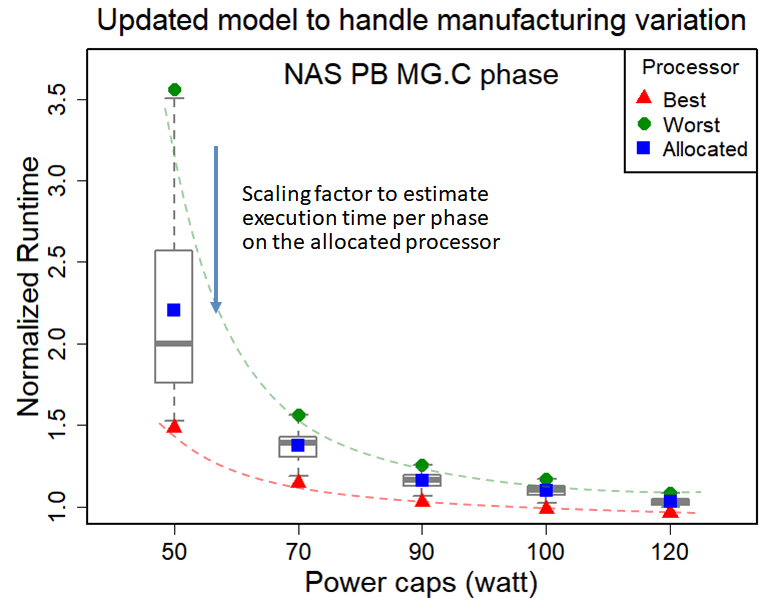
\includegraphics[scale = 0.6]{projects/2.3.1-PMR/2.3.1.12-Power-Steering/power_model.png}
	\caption{Non-linear power-performance model in use for MG.C during configuration exploration phase for the runtime system}
	\label{fig:MG}
\end{figure}


\paragraph{Next Steps}
We will continue our research and development work as planned toward the September 2018 milestones. More specifically, we are working on porting GEOPM to non-Intel architectures (IBM Power8 or Power9, and NVIDIA GPUs are candidates). We will also enhance our variation-aware and phase aware model with advanced machine learning and statistical techniques. We also plan to improve the overhead of the configuration exploration function by selecting configurations that minimize sampling overhead without a significant impact on the prediction accuracy of the power model especially at lower power budgets. 

One of our current challenges is to gain access to non-Intel architectures such as IBM Power8/Power9 and NVIDIA GPUs with elevated privileges that are required for power management. We are working with LLNL to gain such access. Additionally, for our Legion work, we are working toward understanding mappers as well as task distribution better in order to determine the spatial and temporal aspects of power management with GEOPM plugins. We are also looking into S3D application code as part of our Legion power model  exploration. Lastly, we are looking into adding Spack support for installing GEOPM. 

